\documentclass{article}

\usepackage{graphicx}
\usepackage[utf8]{inputenc}
\usepackage[hungarian]{babel}
\usepackage[a4paper, total={5in, 8in}]{geometry}
\usepackage{caption}
\usepackage{subcaption}
\usepackage{float}
\usepackage[hidelinks]{hyperref}

\title{\textbf{Mélytanulás házi feladat dokumentáció}}
\author{Gyömbér Péter, Rikli Szabolcs}
\date{\today}


\begin{document}
	\maketitle
	\newpage
	
	\tableofcontents
	\newpage
	
	\section{A feladat ismertetése}
	
		\par A modern társadalmakban az online közösségi hálózatok, mint például a Facebook, kiemelkedő szerepet játszanak a kapcsolatok kialakításában és fenntartásában. Az ilyen platformok rendelkeznek nagy mennyiségű adattal, amelyek segítségével jobban megérthetjük a felhasználók közötti kapcsolatokat és az ismertségi gráfokat. A jelen feladatban, kidolgoztunk egy modellt, mely a Facebook felhasználók ismertségei alapján, új baráti ajánlásokat készít. A megoldás során a node2vec\footnote{\url{https://arxiv.org/pdf/1607.00653.pdf} \label{node2vec}} gráfbejárási algoritmus segítségével készítettünk beágyazásokat, amik vektorokba kódolják a gráf szerkezeti információit. Ezeket aztán a VGAE (Variational Graph Autoencoder)\footnote{\url{https://arxiv.org/pdf/1611.07308.pdf} \label{vgae}} modell bemenetének szolgáltattunk, hogy azzal új baráti ajánlásokat prediktáljunk. A legjobban teljesítő modell felhasználásával elkészítettünk egy Gradio alkalmazást is, ami az elért eredmények gyakorlati felhasználását mutatja be. 
	
	\section{Adat}
	
		\par Munkánk során a publikusan elérhető „Social circles: Facebook”\footnote{\url{https://snap.stanford.edu/data/ego-Facebook.html}} adatkészletet használtuk, ami az egyes felhasználók közötti kapcsolatokat tartalmazza. Ezt feldolgozva, elkészíthetjük a Facebook hálózat gráf reprezentációját, aminek csomópontja a felhasználók, a köztük lévő baráti kapcsolatokat pedig az élek írják le. Az előállított gráf 4039 csomópontot és 88234 élt tartalmaz. A rendelkezésünkre álló adat kellően jó minőségűnek bizonyult, így kevés feldolgozást kellett végeznünk. Az esetleges többszörös éleket és hurokéleket kiszűrtük a gráfból, ezt használtuk fel a későbbiekben. Néhány statisztikai kimutatást is készítettünk, amik az összefüggések alaposabb megértését segítik. A fokszámok eloszlása (az összes lehetséges kapcsolathoz viszonyítva) például azt mutatja, hogy a felhasználók többsége kevesebb mint 200 kapcsolattal rendelkezik, míg a klaszterezési együttható eloszlás a kapcsolati csomópontok szorosságát szemlélteti. A gráf éleit tanítási, tesztelési és validációs részekre bontottuk, majd csak ezután végeztük el a beágyazások elkészítését.
		
		\begin{figure}[H]
			\centering
			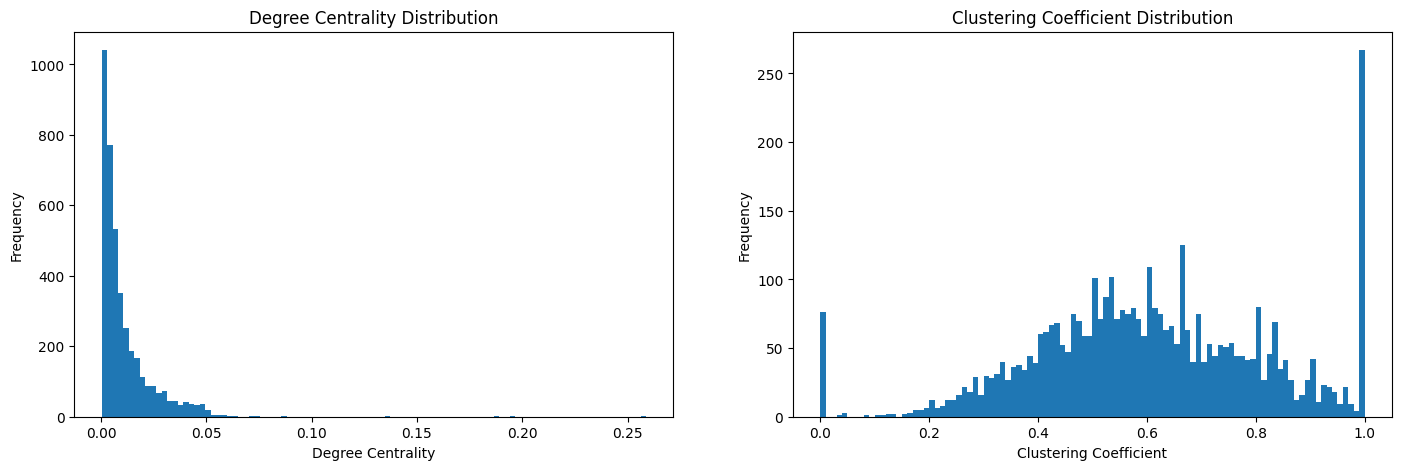
\includegraphics[width=\linewidth]{Figures/analysis.png}
			\caption{Statisztika}
		\end{figure}
	
	\section{Baseline modell}
	
		\par A baseline modellünk a Barabási–Albert-modellben használt \textit{Preferential Attachment} koncepción alapszik. Ez feltételezi, hogy az emberek alkotta nagy hálózatokban (pl. weboldalak hivatkozásai, közösségi hálók) csomósodás figyelhető meg. Az adott rendszert reprezentáló gráfban lesznek kitüntetett csúcsok, akiknek rengeteg szomszédja lesz, viszont a legtöbb maradék csúcsnak viszonylag kevés.
		
		\par A modellünkben először kiválasztjuk a gráfban jelenleg létező élek 80\%-át, ezek alapján fogunk előrejelzést számolni, "tanító adatként" viselkedik. A maradék 20\% a teszt adathalmaz. Hogy a tesztelés alaposabb legyen kiválasztunk a jelenleg nem összekötött élek közül ugyanannyit, mint amennyi él a teszt adathalmazban van.
		
		\par A tanító adatból kiszámoljuk az egyes csúcsok közötti \textit{Preferential Attachment} értékeket egy szomszédsági mátrixba a NetworkX könyvtár segítségével\footnote{\url{https://networkx.org/documentation/stable/reference/algorithms/generated/networkx.algorithms.link_prediction.preferential_attachment.html}}. Fontos megjegyezni, hogy a tanító adatban benne van az összes csúcs, de lehetnek akár elszigeteltek, ha a tanító-tesztelő kiválasztás során nem kerültek be az élei a tanító adatba. A kapott mátrix értékeit lenormáljuk a benne szereplő legnagyobb értékkel, így az értékei egyfajta valószínűségnek foghatóak fel. 0 és 1 közötti értékek, amelyek a kapcsolódás valószínűségét adják meg.
		
		\par A teszt adathalmazban szereplő élek értékeit kiválasztottuk a mátrixból és ezeket hasonlítottuk össze az elvárt értékekkel ami az eredeti gráfban szereplő éleknél 1, a nem létező éleknél pedig 0. Az összehasonlítás a scikit-learn segítségével\footnote{\url{https://scikit-learn.org/stable/modules/generated/sklearn.metrics.roc_auc_score.html}}\footnote{\url{https://scikit-learn.org/stable/modules/generated/sklearn.metrics.average_precision_score.html}} történt.
		
		\par Az így kapott AUC és AC értékek több lefutásra is a 0.8-0.85 értékek között mozogtak.
		
		\begin{figure}[H]
			\centering
			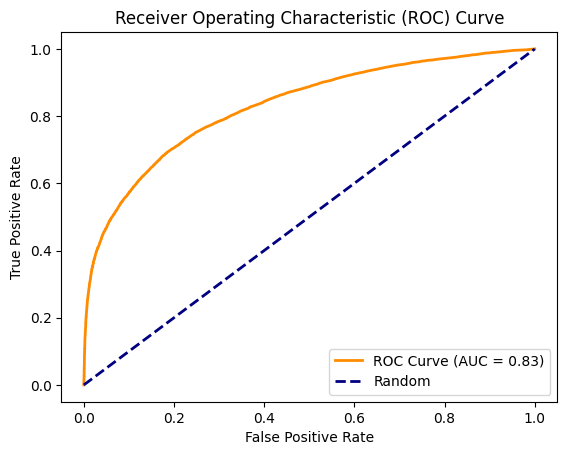
\includegraphics[width=0.6\linewidth]{Figures/baseline_roc_auc.png}
			\caption{Baseline ROC/AUC}
		\end{figure}
	
	\section{Deep learning model}
	
		\par A deep learning modellünk a VGAE cikkben\textsuperscript{\ref{vgae}} ismertetett variációs gráf autoenkóderen alapszik. Ez két részből áll: a csúcs lenyomatok (node embedding) készítése és maga az autoenkóder.
		
		\subsection{Node embedding}
			
			\par Ennek a lépésnek a célja, hogy a gráf csúcsait leképezze egy általunk meghatározott dimenziós térbe és ennek felhasználásával pontosabb eredményt érjen el a neurális hálózat. A csúcs lenyomatokat a node2vec cikkben\textsuperscript{\ref{node2vec}} leírt algoritmussal generáltuk az eredeti gráfból a Pytorch Geometric könyvtár implementációjával\footnote{\url{https://pytorch-geometric.readthedocs.io/en/latest/generated/torch_geometric.nn.models.Node2Vec.html}}. Ennek bizonyos paraméterei bekerültek a modell optimalizálandó hiperparaméterei közé.
			
		\subsection{Input}
		
			\par A bemeneti gráf szét lett bontva tanító, teszt és validációs adatra. Mindhárom halmazhoz lettek generálva negatív élek, amik az eredeti gráfban nem létező éleket jelentik. Ezek száma megegyezik az egyes adathalmazok méreteivel. Mindegyik adathalmaz az eredeti gráfból a node2vec-kel generált mátrixot használja csúcs lenyomatnak.
			
		\subsection{Neurális hálózat}
		
			\par A modellünk a Pytorch Geometric VGAE osztályát\footnote{\url{https://pytorch-geometric.readthedocs.io/en/latest/generated/torch_geometric.nn.models.VGAE.html}} használja alapnak, vagyis ebből származik le. Ez egy variációs gráf autoenkóder alaposztály. Ehhez nekünk csak egy enkódert, egy dekódert és egy kiegészített loss függvény kellett írnunk.
			
			\par A dekódert igazából nem kellett megírnunk, mert a könyvtárban van előre megírt dekóder\footnote{\url{https://pytorch-geometric.readthedocs.io/en/latest/generated/torch_geometric.nn.models.InnerProductDecoder.html}} a VGAE osztályhoz, ami nekünk jó volt és nem kellett kiegészítenünk.
			
		\subsection{Hiperparaméter optimalizáció}
		
			\par Az optimalizációt Weights \& Biases-zel csináltuk. Minden egyes futásra új bemenet lett generálva. A dockeren való bejelentkezést megspórolva a kódba égettük az egyikünk wandb API kulcsát és ezt használja futáskor a modell. Miután a sweep lefutott a legkisebb validációs losshoz tartozó hiperparamétereket betölti és azzal tanítja be a végleges modellt. A hozzá tartozó online felületen több információ is megtalálható a hiperparaméterekről\footnote{\url{https://wandb.ai/szabolcsrikli/Deep\%20Learning\%20Homework?workspace=user-szabolcsrikli}}.
	
	\section{Kiértékelés}
	
		\par A tanítás eredményének kiértékelésére többféle metrikát is használunk. Először is meghatározzuk a ROC és Precision értékeket, amik a tanulás során folyamatosan nyomon követhetők a veszteséggel együtt. Ezek jól leírják, hogy a rekonstruált gráf milyen mértékben volt képes visszaállítani az eredetit. Ezenfelül elkészítjük a predikciós szomszédsági mátrixot, ami tartalmazza az összes lehetséges él létezésének a valószínűségét. Utána ezt összevetjük az eredeti gráffal és azt vizsgáljuk, hogy a prediktált élek hogyan viszonyulnak az eredetileg létezőkhöz. Itt figyelünk arra, hogy a pozitív és negatív élek száma megegyezzen. Majd a predikciókat és a tényleges címkéket összehasonlítva szintén számolunk egy ROC görbét és ki is rajzoltatjuk azt.
		
		\begin{figure}[H]
			\centering
			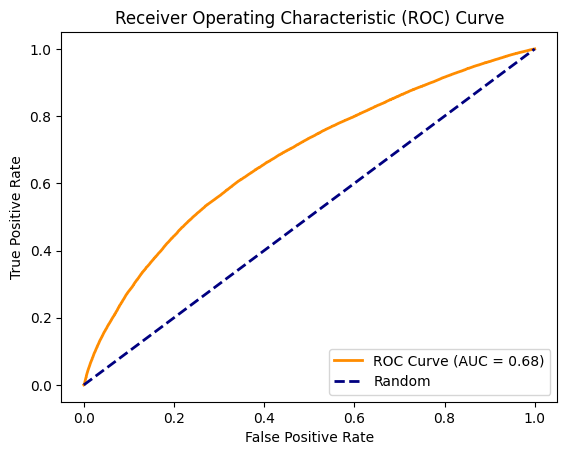
\includegraphics[width=0.6\linewidth]{Figures/model_roc_auc.png}
			\caption{Model ROC/AUC}
		\end{figure}
	
		\newpage
		\subsection{Gradio}
		
			\par Az adat analízis és a két modell végeredménye egy Gradioval készített felületen elérhető a futás végén. Meg kell adnunk a csúcs sorszámát, aminek kíváncsiak vagyunk a javaslataira és a "Run" feliratú gombra kattintva megjelenik a 10 legvalószínűbb összeköttetés. Emellett megjelenik az adott csúcshoz tartozó összes jóslat valószínűségének eloszlása.
			
			\begin{figure}[H]
				\centering
				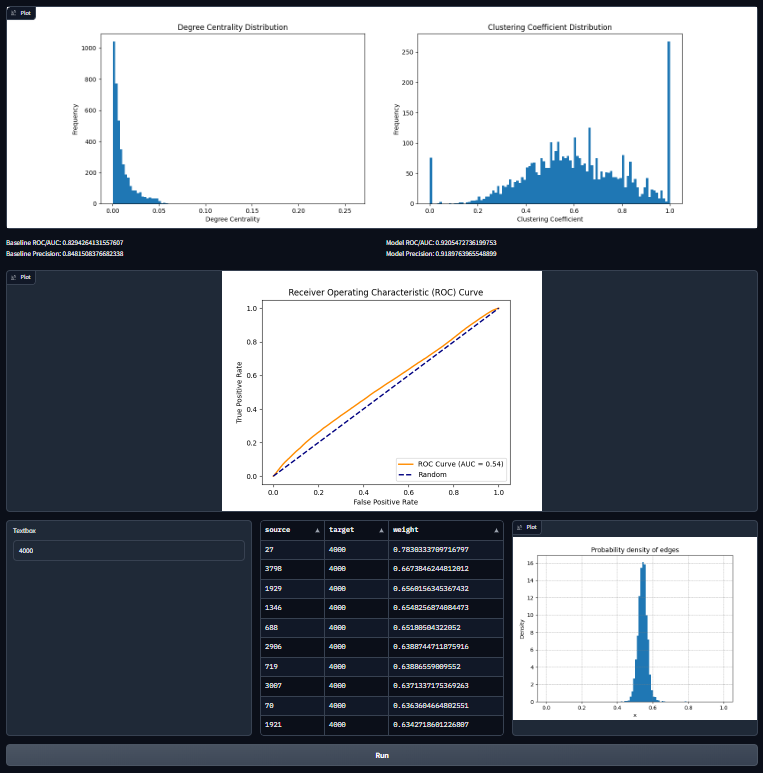
\includegraphics[width=\linewidth]{Figures/gradio.png}
				\caption{Gradio felület}
			\end{figure}
	
	\section{Konklúzió}
	
		\par Az általunk felhasznált facebook adathalmazban az összes 8154741 db potenciális élre kaptunk a modelltől előrejelzést az adott összeköttetés bekövetkezési valószínűségére. Az eredeti gráf esetén nagyon sok élre 50\% körüli értékeket kaptunk, de ha hozzáadtunk éleket véletlenszerűen a gráfhoz és így tanítottuk a modellt, akkor az összeköttetések jóslásában egyre magabiztosabb lett a modell. A 0.5-ből egyre jobban eltolódtak a 0 és 1 értékek felé a becsült valószínűségek. Ebből arra következtetünk, hogy több csúcsot és élet tartalmazó gráfok esetén a modellünk jobb eredményt adhat.
		
		\begin{figure}[H]
			\centering
			\begin{subfigure}[H]{0.49\textwidth}
				\centering
				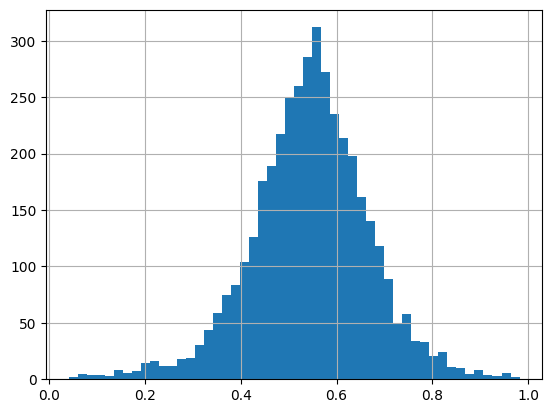
\includegraphics[width=.9\textwidth]{Figures/few_edges.png}
				\caption{Eredeti gráf}
			\end{subfigure}
			\begin{subfigure}[H]{0.49\textwidth}
				\centering
				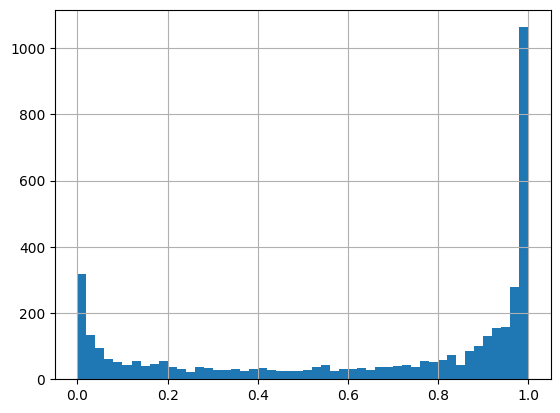
\includegraphics[width=0.9\textwidth]{Figures/many_edges.png}
				\caption{Hozzáadott élekkel}
			\end{subfigure}
			\caption{Élek valószínűségének eloszlása}
		\end{figure}
		
		\par Próbáltuk lefuttatni nagyobb gráfokon (Google+ és Twitter példák), de a rendelkezésünkre álló Google Colab Pro által nyújtott 52 gb RAM elfogyott mindegyik esetben és crashelt, tehát nem tudtuk kipróbálni a modellt nagyobb hálózatokra.
\end{document}